\chapter{基础网络的研究与选择}

\section{主流基础网络特性分析}
目前情况下,包括图像检索在内的许多计算机视觉任务,在大部分情况下都会使用常用的基础分类网络作为其骨干网络充当特征提取器,这些主流的分类网络的性能已经在ImageNet得到证明。最经典的卷积神经网络是Yann LeCun在1998年设计并提出LeNet,这个用于识别手写字符的网络规模较小,但是包含了现在卷积神经网络的最基本组件:卷积层,池化层,全连接层。Alex Krizhevsky于2012年提出的AlexNet是卷积神经网络的一大步:AlexNet使用ReLU取代Sigmoid作为激活函数,成功解决了Sigmoid在网络较深时的梯度弥散问题;训练时采用了Dropout策略,随机忽略一部分神经元,可以有效避免模型的过拟合;引入了最大池化层而不是像之前只使用平均池化层,这有效的提升了特征的丰富性;使用CUDA加速神经网络训练,有效利用了GPU的计算能力。AlexNet被提出之后,深度学习飞速发展,越来越多性能优异的基础网络随之被提出,下面简要分析几个主流的基础网络:
\begin{itemize}
  \item [1.]VGG:相比AlexNet,VGG的一个改进是采用连续的几个3x3的卷积核代替AlexNet中的11x11或者5x5的较大卷积核。对于给定的感受野,采用堆积的小卷积核是优于采用大的卷积核,因为多层非线性层可以增加网络深度来保证学习更复杂的模式,此外小的卷积核也意味着更少的参数量,更低的计算复杂度。总结性的来说,VGG在控制计算量增长的同时将网络架构做的更深更宽,分类效果显著提升。\begin{figure}[h]
  \centering
  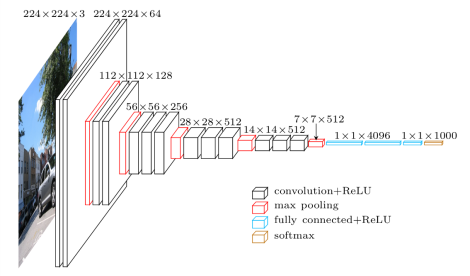
\includegraphics[width=10cm, height=6cm]{Img/vgg.png}
  \caption{VGG整体结构}
  \label{fig:vgg}
\end{figure}

\item [2.]Inception:又被称为GoogLeNet,实际上Inception指的是GoogLeNet的核心结构。一般来说提高网络表达能力最直接的方法就是增加网络的深度和宽度,但是直接这么做会带来一些问题:
\begin{itemize}
  \item [(1)]相对更深更宽的网络不可避免的会增加参数量,而过多的参数量容易导致过拟合。
  \item [(2)] 随着网络的深度的增加,反向传播时会出现梯度消失的问题,导致网络很难优化。
  \item [(3)] 计算量增加,会消耗更多的计算资源。
\end{itemize}

Inception结构针对限制神经网络性能的主要问题对传统的卷积策略不断改进,Inception v1设计出了多路并行的卷积模块,不同分支的卷积核大小不同,分别有1x1,3x3,5x5三种尺度,这么做的好处是可以以不同大小的感受野去学习得到不同的特征,卷积操作之后,不同分支的特征通过拼接的方式做融合。
\begin{figure}[h]
  \centering
  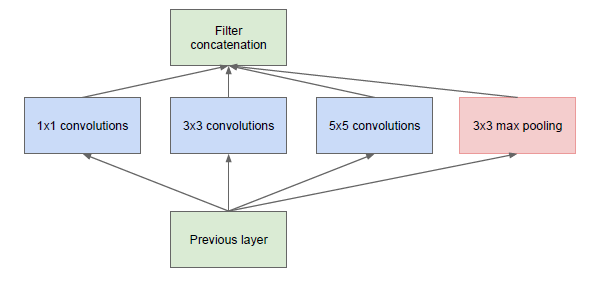
\includegraphics[width=13cm, height=6cm]{Img/inception-v1.png}
  \caption{Inception v1}
  \label{fig:inception-v1}
\end{figure}

Inception v2\cite{ioffe2015batch}基于Inception v1做了进一步的改进,提出了有重大意义的BN(Batch Normalization)。训练深度神经网络时,作者抛出一个叫做“Internal Covariate Shift”的问题,这个问题指在训练过程中,第n层的输入就是第n-1层的输出,在训练过程中,每训练一轮参数就会发生变化,对于一个网络相同的输入,但n-1层的输出却不一样,这就导致第n层的输入也不一样,BN的提出就是为了解决这个问题。在传统机器学习中,对图像提取特征之前,都会对图像做白化操作,即对输入数据变换成0均值、单位方差的正态分布,卷积神经网络的输入就是图像,白化操作可以加快收敛,对于深度网络,每个隐层的输出都是下一个隐层的输入,即每个隐层的输入都可以做白化操作,BN就是在训练中的每个mini-batch上做了白化,可以有效防止梯度消失并加速网络训练。

\item [3.]ResNet:由微软研究院的Kaiming He等提出的ResNet,通过使用ResNet Unit成功训练出了152层的神经网络,其效果非常优异,在ILSVRC2015比赛中夺得头筹。

提出残差学习的思想。传统的卷积网络或者全连接网络在信息传递的时候或多或少会存在信息丢失,损耗等问题,同时还有导致梯度消失或者梯度爆炸,导致很深的网络无法训练。ResNet在一定程度上解决了这个问题,通过直接将输入信息绕道传到输出,保护信息的完整性,整个网络只需要学习输入、输出差别的那一部分,简化学习目标和难度。VGGNet和ResNet的对比如下图所示。ResNet最大的区别在于有很多的旁路将输入直接连接到后面的层,这种结构也被称为shortcut或者skip connections。

\begin{figure}[h]
  \centering
  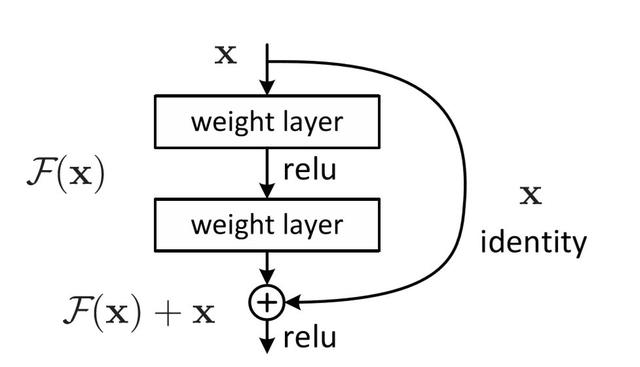
\includegraphics[width=10cm, height=6cm]{Img/resnet.jpg}
  \caption{ResNet 残差模块\cite{he2016deep}}
  \label{fig:resnet}
\end{figure}


\item [4.]SENet:近年来,为了提升网络性能,多数工作从空间纬度展开,比如Incepion使用
多尺度的卷积核以获取并聚合不同感受野的特征,另外比较具有代表性的有将注意力机制
引入到空间维度上去,这些工作都取得了很好的效果。而SENet则引入了另一种思路:是否可以考虑特征通道之间的关系以提升网络性能?SE是Squeeze-and-Excitation的缩写,
Squeeze和Excitation则是SENet核心模块的两个关键操作,模块具体流程如下:
\begin{itemize}
  \item [(1)] 对一个三维的特征图做Global average pooling,得到特征维度为${c\times1\times1}$,其中c为特征图的通道数,这个操作成为Squeeze。
  \item [(2)] 随后为两个FC层(Fully-connected-layer)去学习通道之间的相关性,其中第一个FC层将输入维度降低至原来的1/16,并经过ReLu,第二个FC层再将特征升至原来的维度。
  用两个FC层的好处是可以增加非线性以更好的建模通道相关性,并且可以大幅度减少参数量。
  \item [(3)] 最后通过Sigmoid将特征归一化至0到1之间,代表每个通道的重要程度,并将权重点乘至原特征图上。
\end{itemize}
\end{itemize}
\begin{figure}[h]
  \centering
  \includegraphics[width=12cm, height=6cm]{Img/backbone.pdf}
  \caption{基于基础网络的简单检索网络}
  \label{fig:backbone}
\end{figure}


\section{SE-Inception}
